%!TEX root = ../Thesis.tex

\chapter{Test and Results}
This chapter deals with testing of the prototype, discussion of the results achieved and how to improve the results in case the data achieved is not satisfying.  

\section{The test setup}
Given to the short time frame for this project and unexpected long time sick leave foreman in the mechanical workshop some short cuts was performed in order to get a working prototype. The mechanical and electrical parts are fitted into a rack cabinet.

\begin{figure}[hbtp]
  \centering
  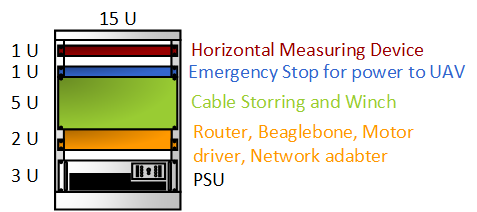
\includegraphics[scale=1]{graphics/Visio/rack-setup.png}
  \caption{Rack cabinet overview.}
  \end{figure}   

\noindent
From top the Horizontal Measurement Device is mounted underneath the helipad. On the front a emergency switch is mounted to disconnect the 75 volt supply to the UAV. In the middle there is room for cable storing and winching mechanism. The position of the winch can easily be adjusted through aluminium bars milled track.
\todo{Indsæt billede}
Underneath that a shelf is mounted with the Beaglebone, motor driver, Network adapter and router.
At the bottom, the DC/DC power converters are mounted and a on/off switch is surface mounted to the entire system.  

\section{Cable Drum}
To address the heating issue in the cable drum a test was performed to evaluate the heating’s influence, in order to incorporate the results in the design process.\\

\subsection{Test - Worst-case heating in cable}
The worst-case test with full load over long time was performed at indoor environment with room temperature on 24 degree Celsius. The coil was excited with 75V DC and 360W just over an hour. This is not 100 per cent of the UAVs power consumption, but the testing equipments upper limit. The inner diameter of the coil is 10cm and is made of 2mm thick PVC pipe.


\begin{figure}[H]
   \centering
   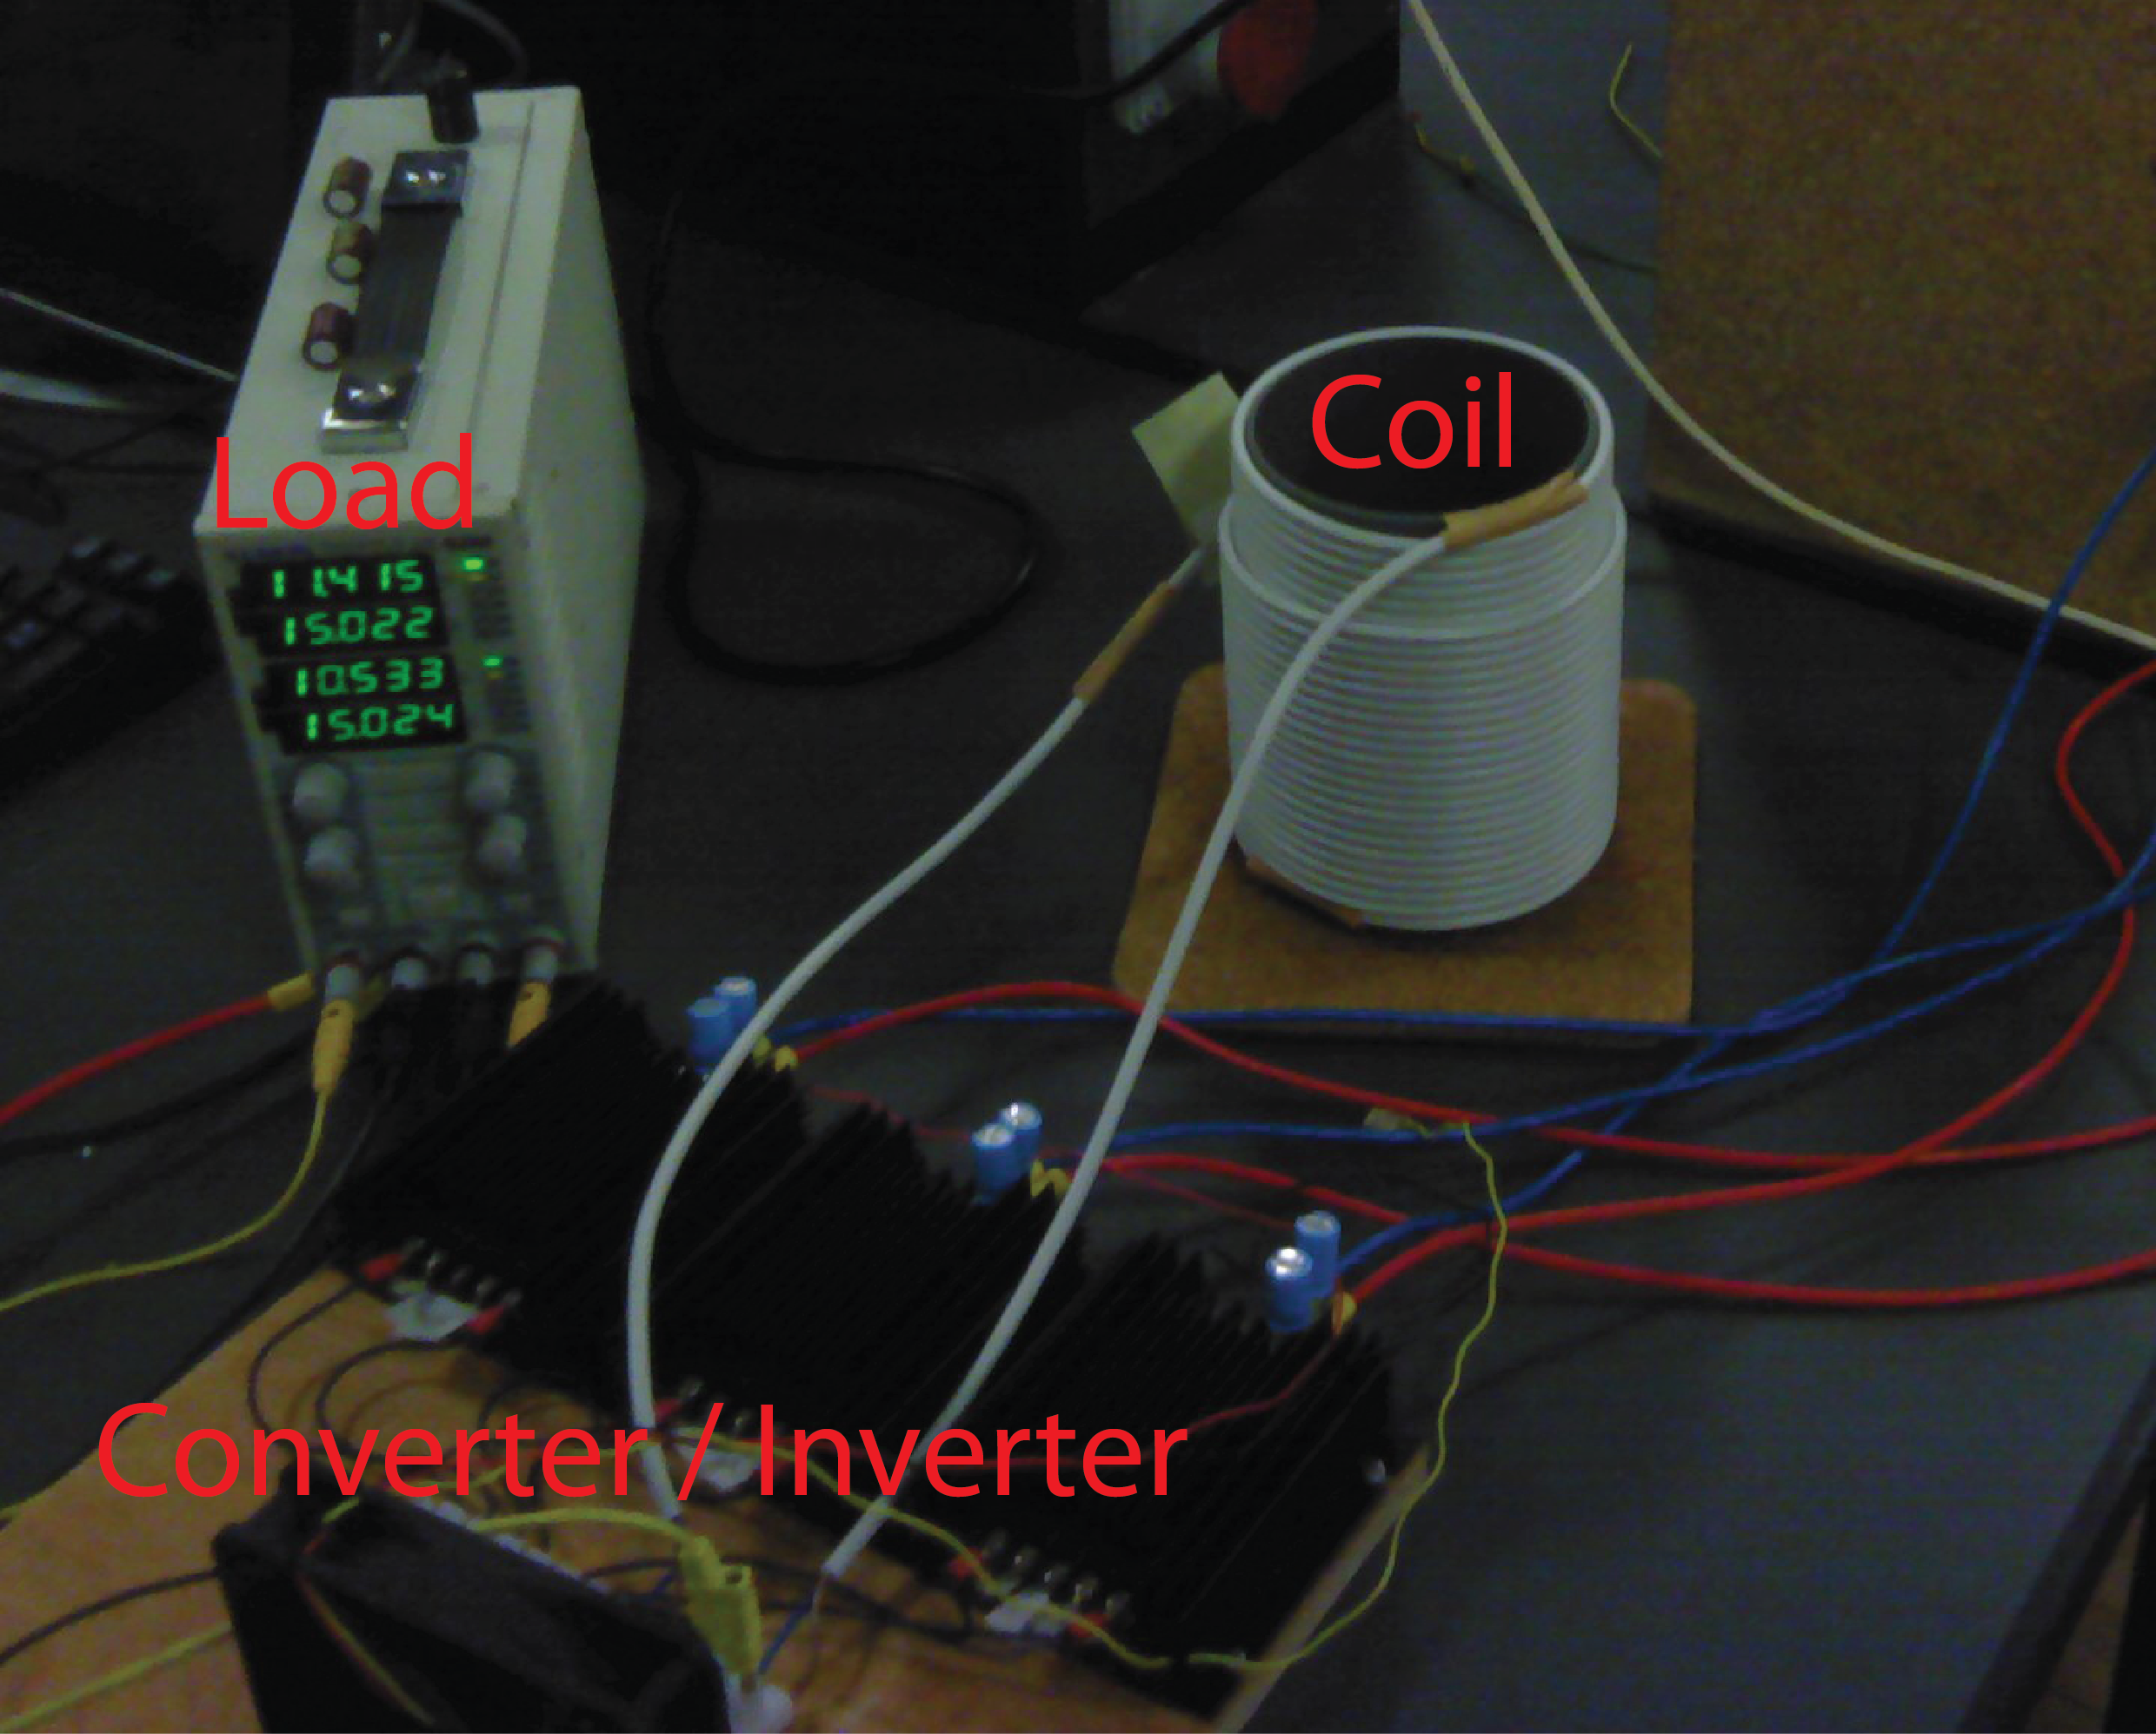
\includegraphics[scale=0.5]{graphics/heat_test/heat_test_setup.png}
   \caption{Heat test setup showing the coil, the test load and DC/DC power converters.}
   \end{figure}
      

\begin{figure}[H]
\centering
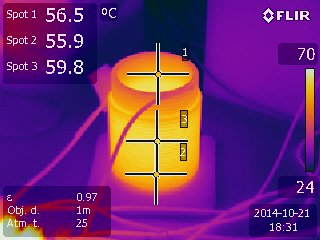
\includegraphics[scale=1]{graphics/heat_test/IR_1491.jpg}
\caption[Heat test, image from thermal camera]{Heat test of 20m standard household cable\footnotemark winded in two layers with 75V DC and 360W. Spot 1 is inside the coil, spot 2 is the lower side of the outer coil and spot 3 i at center of the outer coil. On the lower left corner thermometer calibration constants is displayed.}
\label{fig:heat_test_ir}
\end{figure}
\footnotetext{House hold cable with unknown origin, cross-sectional area 0.75mm2, Max voltage 230 AC, Max current 10A}

\subsection{Summary}
Even through the cable is not excited with 100 per cent of the UAV power consumption; the test puts the heating issue in perspective. The heating is not critical high, but must be considered in the cable requirement specification; hence, CE certification only requires the cable to withstand up to 80 degrees\cite{Parliament2006}.    



\section{Horizontal Measuring Device}
This measurement devices is tested with regards to stability and the results of the calculated position references. Hence this is relative cheap load cells, the precision is expected to be with in an acceptable region.

\subsection{Calibration}
First off is calibrating the load cells. First measurement is without any forces acting in $x$ and $y$ direction in order to determine the offset of each load cell.
The offset for $x$ is found to $-455.9787$ and the $y$ offset to $-511.2618$, as seen on figure \ref{fig:HMDcalib}.\\

\begin{figure}[hbtp]
\centering
\includegraphics[scale=1]{graphics/gcs_test/calib_0_data_raw.eps}
\caption[Raw data from load cell]{Raw input data from load cell $x$ and $y$. The average line is the calculated offset used for calibration. Measured without load any directions.}
\label{fig:HMDcalib}
\end{figure}

\noindent
Next 1000g of load is put on the load cell with a rope through the Teflon ring first purely in positive $x$ direction and next in purely $y$ direction, in order to determine the gain factor $Kx$ and $Ky$. $Kx$ is found to $0.4786$ and $Ky$ to $-0.5134$. Afterwards the calibration is tested by applying $600$g of force in $x$-direction and then checking the result.

\begin{figure}[hbtp]
\centering
\includegraphics[scale=1]{graphics/gcs_test/calib_result_compare.eps}
\caption[Comparing raw data from load cells to the calibrated values]{Comparing raw data to the calibrated values. The $x$-calibrated values are between $633$g and $636$g, then the force applied was $600$g. The $33-36$g difference is most likely caused by the limitations of precision from the spring load. The y-calibrated data is ranging from $-29$g to $-32$g. It is expected the precision can vary $\pm75$g around the zero balance.}
\end{figure}

\newpage
\subsection{Test of calibration}
After the calibration process, a test of the calibration shows the quality of the calibration.
This test is performed by applying a known force in a combination of $x$ and $y$ direction. For this test $\phi$ is set to 45 degrees and the total force is $1$kg. On figure \ref{fig:phi45deg1kg} it is seen that the data slightly decreases over time. This is probably due to tolerances in the manufacturing process of the mount enabling the load cell to move slightly over time or the elasticity of the connecting rope between the spring load and the load cell.

\begin{figure}[hbtp]
\centering
\includegraphics[scale=0.8]{graphics/gcs_test/phi45deg1kg.eps}
\caption[Test combines both $x$ and $y$ direction]{This test combines both $x$ and $y$ direction, therefore the force is calculated into the variable $r$, equivalent to $T_0$ from the analysis chapter. Notating at around $1$kg of load the data drift slightly decreasing.}
\label{fig:phi45deg1kg}
\end{figure}

\newpage
\noindent
On figure \ref{fig:phi45deg1kg} it is seen that the data slightly decreases overtime. This is probably due to tolerances in the manufacturing process enabling the load cell to move slightly over time or it can be caused by the spring load is permanently bending. Taking a closer look at the data on figure \ref{fig:phi45deg1kgdata} showing this phenomena applies to both $x$ and $y$ load cell. Because it applies to both load cells the calculated angle $\phi$ is constant, thus the drift the data is still valid and results in an accurate angle.

\begin{figure}[hbtp]
\centering
\includegraphics[scale=0.8]{graphics/gcs_test/phi45deg1kgdata.eps}
\caption[Calibrated data from $x$ and $y$ load cell]{Showing the calibrated data from $x$ and $y$ load cell then 1kg of load is applied with $\phi=45$ degrees.}
\label{fig:phi45deg1kgdata}
\end{figure}


\newpage
\subsection{Testing with $\theta>0$}
Next test is performed by keeping the $\phi$ angle and the tension constant and varying the $\theta$ angle. Is is expected as $\theta$ approach $90$ degrees the measured force will be approaching $0$. 
\begin{figure}[hbtp]
\centering
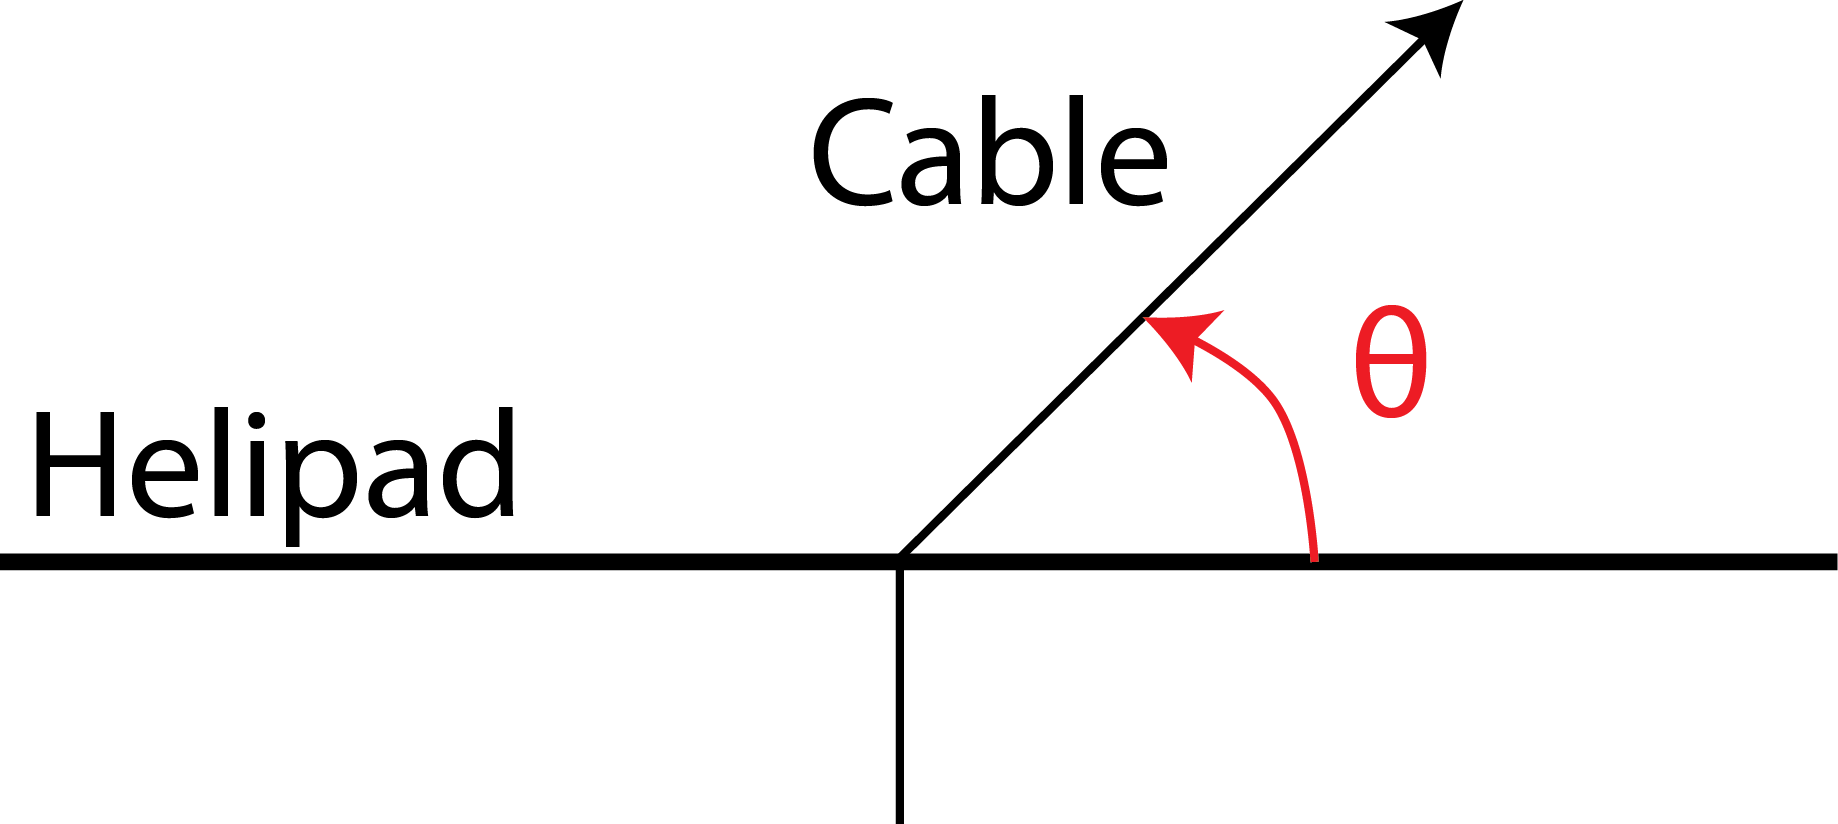
\includegraphics[scale=0.75]{graphics/loadcell_test2.png}
\caption{Testing the horizontal measuring device by keeping $\phi$ constant and varying $\theta$.}
\label{fig:loadcell_test2}
\end{figure}

\noindent
At $\theta=45$ degrees and 1kg of load the measured result is very close to the expected result.

\begin{figure}[hbtp]
\centering
\includegraphics[scale=1]{graphics/gcs_test/45degTheta1kg.eps}
\caption[Comparing the measured load to the theoretical value]{Comparing the measured load to the theoretical value. Showing slightly less than expected.}
\label{fig:45degTheta1kg}
\end{figure}

\noindent
At all previous tests the load has only been anchored in the Teflon ring, but in the real setup the cable are anchored in the winch instead. This mean the measured force is now only a component of the total force. From figure \ref{fig:catenary_force_diagram} $T_0$ only has an x-component, but when the cable now is anchored in the winch the total force equation change to:

\begin{equation}
\sum T -\lambda gs + (T_{0,x} + T_{whinch,y} ) = 0
\end{equation}

\noindent
Hence the measurement device only measures $T_{0,x}$, $T_{whinch,y}$ is unknown. This test will show how much $T_{winch,y}$ influences.
On figure \ref{fig:45degTheta1kg} the measured values are slightly higher than expected. At $\theta = 0$ the overshoot is $13-17$g and at $\theta = 45$ the overshoot is $28-32$g, which is within what's in the first test was discussed as due to limitation in precision of the calibration. 



\newpage
\subsection{Summary}
The prototype is able to measure the force in $x$- and $y$-direction, $\phi$ and $r$ can be calculated with good results. Higher precision might be possible with more precise testing equipment.
The 5kg load cell has a zero balance at $\pm75g$. Any values close to this range must be considered as very unreliable. 
When calibrating the 5kg load cell, the calibration gives better results using a calibration load greater than $0.5$kg.
The force in $T_{winch,y}$ is quite small and can therefore be ignored.\\
All plots have a zoom time axis, thus resulting in more readable and intuitive graphics. All test where measured in 60-120 seconds to ensure the data is stable over time.

\newpage
\section{Tree Dimensional Force Measurement Device}
This measurement devices consist of tree load cells, all perpendicular to each other. The load cells are of different working range, but after calibration their scale is close to equal. However they have different precision, creep and non-linearity region, which might cause unexpected results.

\subsection{Calibration}
As in the Horizontal Measuring Device, first thing is to perform a calibration, now in tree axes, but with same method. The $x$ offset is $-5992.5241$, $y$ offset $464.4041$, and $z$ offset $104.0533$, as seen on figure \ref{fig:fcs-calib-offset}.\\

\begin{figure}[hbtp]
\centering
\includegraphics[scale=1]{graphics/fcs_test/fcs_calib.eps}
\caption[Raw input data from load cell $x$, $y$, and $z$.]{Raw input data from load cell $x$, $y$, and $z$. The average line is the calculated offset used for calibration. Measured without any load.}
\label{fig:fcs-calib-offset}
\end{figure}

\noindent
The $z$-axis is calibrated with 1000g load, hence it is a 5kg load cell. The $x$- and $y$-axes is calibrated with 500g load, hence their measuring range limit is $0.78$kg. The gain is calculated to: $Kx=0.0868$, $Ky=-0.0851$, and $Kz=0.4277$. 
\\

\newpage
\subsection{Test of Calibration}
Testing the calibration with 600g of load at $\phi=0$ degrees and $\theta=45$ degrees. The results are shown on figure \ref{fig:FCS-calib-results}. The results seams to have unexpected results in the first 10 seconds and the last 20 seconds. This might be due to vibrations in the test setup, when people are walking by, touching the table, or the spring is not in equilibrium, because the distortion is seen on all tree axes. From approximate 15 seconds in to 50 seconds, the reading is quite stable, thus it has a slight drift. This drift is, as describes in testing of the Horizontal Measurement Device, presumably given due to elasticity in the rope, the spring is permanently bending or tolerances in the manufacturing process gives rise to small displacements of mechanical components.\\
\\

\begin{figure}[hbtp]
\centering
\includegraphics[scale=1]{graphics/fcs_test/calib_result_compare.eps}
\caption{d}
\label{fig:FCS-calib-results}
\end{figure}

\todo{Lav plot af de beregnede vinkler osv.}

\subsection{Summary}
\todo{Lav en opsummering}



\newpage
\section{Data Connection test}
The data connection is tested by performing a ping test from Ground Control Station to the Flight Control Station and measuring the response time. The ping test is started and then the throttle for the UAV is moved slowly up to a point where the UAV is close to take off.

\begin{figure}[hbtp]
\centering
\includegraphics[scale=1]{graphics/pingTest.eps}
\caption{Ping test from Ground Station to Flight Control Station, while throttle is on.}
\label{fig:pingTest}
\end{figure}

\noindent
From figure \ref{fig:pingTest} the average response time is $5.16$ms which is a robust result. Unfortunately is have not been possible to test the data connection when the UAV is on full throttle, which also is the worst-case conditions for the network connection. The test where performed with 50m of cable, and the supply volte in the power line never went under 69 volt. Taking this in consideration further testing must be performed to finally conclude if this concept works. 


